\chapter{Randomized Algorithms}
\label{ch:randomized}
\label{ch:randomization}
{ 

\newcommand{\qsort}{quicksort}
\newcommand{\Qsort}{Quicksort}

\newcommand{\SSpace}{\ensuremath{\Omega}}
\newcommand{\EventE}{\mathcal{E}}

The theme of this chapter is $\overset{\mbox{\em
    randomized}~~~~~~}{\mbox{\em \st{madendrizo} algorithms}}$.  These are
algorithms that make use of randomness in their computation.  You
might know of \qsort, which is efficient on average when it uses a
random pivot, but can be bad for any pivot that is selected without
randomness.

Even though analyzing randomized algorithms can be difficult,
randomization turns out to be a crucial technique for algorithm
design, making the extra effort well worth. 
%
For example, for some problems randomized algorithms are simpler or
faster than non-randomized algorithms. 
%
The problem of primality testing (PT), which is to determine if an
integer is prime, is a good example.  In the late 70s Miller and Rabin
developed a famous and simple randomized algorithm for the problem
that only requires polynomial work.  For over 20 years it was not
known whether the problem could be solved in polynomial work without
randomization.  Eventually a polynomial time algorithm was developed,
but it is much more complicated and computationally more costly than
the randomized version.  Hence in practice everyone still uses the
randomized version.

\begin{comment}
fun checkPrime(n, k) = 
let
     fun sAndD (s,d) =
       if isOdd(d) then (s,d)
       else sAndD(s+1,d/2)
     val (s,d) = sAndD(0,n)

     fun sample(k) = 
       if (k = 0) then ProbPrime 
       else let
         val a = random(2,n-2)
         val x = a^d \mod n
         fun trySquares(x,s) =
             if (x = 1 orelse s = 0) then Composite
             else if (x = n -1) then ProbPrime
             else trySquares(x^2 \mod n,s-1)
       in
          if (x = 1 orelse x = n-1) then sample(k-1)
          else if (try(x,s-1) = ProbPrime) then sample(k-1)
          else Composite
       end
in
     sample(k)
end
\end{comment}

There are many other problems in which a randomized solution is
simpler or cheaper than the best non-randomized solution.  In this
chapter, after covering the prerequisite background, we will consider
some such problems.  The first we will consider is the following
simple problem:
\begin{quote}
  \textbf{Question:} How many comparisons do we need to find the top two 
largest numbers in a sequence of $n$ distinct numbers?
\end{quote}
Without the help of randomization, there is a trivial algorithm for
finding the top two largest numbers in a sequence that requires about
$2n - 3$ comparisons.  We show, however, that if the order of the
input is randomized, then the same algorithm uses only $n + O(\log n)$
comparisons in expectation (on average).  This matches a more
complicated deterministic version based on tournaments.

Randomization plays a particularly important role in developing parallel
algorithms, and analyzing such algorithms introduces some new
challenges.  
%
In this chapter we will look at two randomized algorithms with
significant parallelism: one for finding the $k^{th}$ order statistics
of a sequences, and the other is \qsort.  In future chapters we will
cover many other randomized algorithms.

In this book we require that randomized algorithms always return the
correct answer, but their costs (work and span) will depend on random
choices.  
%
Such algorithms are sometimes called \defn{Las Vegas algorithms}.
Algorithms that run in a fixed amount of time, but may or may not
return the correct answer, depending on random choices, are called
\defn{Monte Carlo} algorithms.


\section{Expectation versus High Probability}
\label{sec:randomized::probability}

In analyzing costs for a randomized algorithms there are two types of
bounds that are useful: expected bounds, and high-probability bounds.
%

\begin{todo}
Develop an example here.  I think what you need is to have n tasks
each of which require 1 time with probability (m-1)/m and m time with
probablity 1/m.  you can show that the span is almost alway m by
choosing n to be large.
\end{todo}


\defn{Expected bounds} tell us about the average cost across all
random choices made by the algorithm.  
%
For example if an algorithm has $\Theta(n)$ expected work, it means that on
averaged over all random choices it makes in all runs, the algorithm
performs $\Theta(n)$ work.
%
Since expected bounds are averaged over all random choices in all
possible runs, there can be runs that require more or less work.
%
For example
%
once in every $1/n$ tries the algorithm
might require $\Theta(n^2)$ work, 
%
and (or)
%
once  in every $\sqrt{n}$ tries the algorithm might require
$\Theta(n^{3/2})$ work.


\defn{High-probability} bounds on the other hand tell us that it is
very unlikely that the cost will be above some bound.  
%
For a problem of size $n$ we say that some property is true with high
probability if it is true with probability $1 - 1/n^k$ for some
constant $k > 1$.  
%
This means the inverse is true with very small
probability $1/n^k$.
%
Now if we had $n$ experiments each with inverse probability $1/n^k$ we
can use the union bound to argue that the total inverse probability is
$n \cdot 1/n^{k} = 1/n^{k-1}$.  This means that for $k > 2$ the
probability $1 - 1/n^{k-1}$ is still true with high probability.
%
High-probability bounds are typically stronger than expectation
bounds.


Expected bounds are quite convenient when analyzing work (or
running time in traditional sequential algorithms).  
%
This is because the linearity of expectations (\chref{probability})
allows adding expectations across the components of an algorithm to
get the overall expected work.
%
For example, if the algorithm performs $n$ tasks each of which take on
average $2$ units of work, then the total work on average across all tasks will
be $n \times 2 = 2n$ units.
%
Unfortunately this kind of composition does not work when analyzing
the span of an algorithm, because this requires taking the maximum of
random variables, rather than their sum.
%
For example, if we had $n$ tasks each of which has expected span of
$2$ units of time, we cannot say that the expected span across all
tasks is $2$ units.
%
It could be that most of the time each task has a span of $2$ units,
but that once with probability $1/n$,  the task requires $n$ units.
%
The expected span for each task is still close to $2$ units but if we
have $n$ tasks chances are high that one task will take $n$ units and
the expected maximum will be close to $n$ rather than $2$.
%
We therefore cannot compose the expected span from each task by taking
a maximum.
%


Unlike expected bounds, high-probability bounds can allow us to bound
span.
%
For example, lets say we know that every task finishes in $2$ units of
time with probability $1 - 1/n^5$, or equivalently that each task
takes more than $2$ units of time with probability $1/n^5$ and takes
at most $n$ units of time otherwise.
%
Now with $n$ tasks the probability that there will be at least one
that requires more than $2$ units of time is at most $1/n^4$ by union
bound.
%
Furthermore, when it does, the contribution to the expectation is
$1/n^3$.
%
Because of these properties of summing vs. taking a maximum, in this
book we often analyze work using expectation, but analyze span using
high probability.

\begin{figure}
\begin{center}
\framebox{
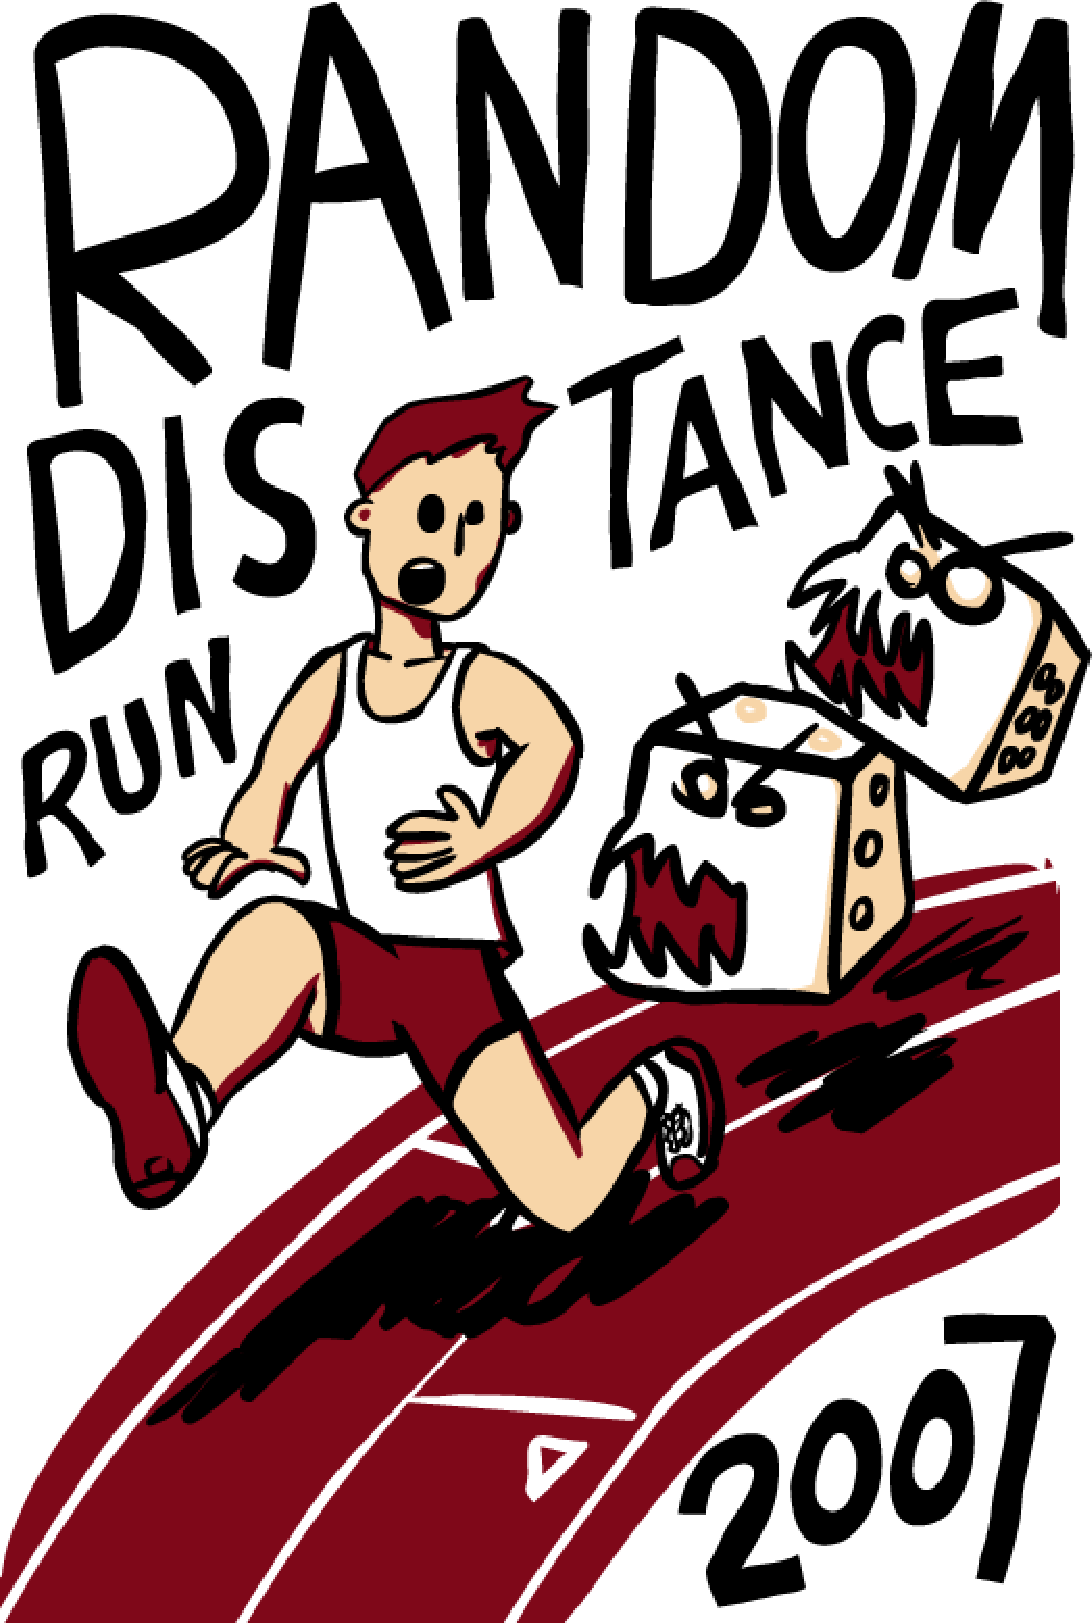
\includegraphics[width=2.3in]{./randomized/rdr.pdf}
}~~~~~
\begin{minipage}[b]{2.8in}
\caption{Every year around the middle of April the Computer Science
  Department at Carnegie Mellon University holds an event called the
  ``Random Distance Run''.  It is a running event around the track,
  where the official dice tosser rolls a dice immediately before the
  race is started.  The dice indicates how many initial laps everyone
  has to run.  When the first person is about to complete the laps, a
  second dice is thrown indicating how many more laps everyone has to
  run.  Clearly, some understanding of probability can help one decide
  how to practice for the race and how fast to run at the start.
  Thanks to Tom Murphy for the design of the 2007 T-shirt.}
\label{fig:rdr}
\end{minipage}
\end{center}
\end{figure}






%% We now consider how to derive high-probability bounds.  We can start
%% by considering the probability that when flipping $n$ unbiased coins
%% all of them come up heads.  This is simply $1/2^n$ since the
%% sample space is of size $1/2^n$, each primitive event has equal
%% probability, and only one of the primitive events has all heads.
%% Certainly asymptotically $1/2^n < 1/n^k$ so the fact that we will not
%% flip $n$ heads is true with high probability.  Even if there are $n$
%% people each flipping $n$ coins, the probability that no one will flip
%% all heads is still high (at least $1 - n/2^n$ using the union bound).

%% Another way to prove high-probability bounds is to use Markov's
%% inequality.  As we will see in Section~\ref{sec:kthsmallest} it is
%% sometimes possible to bound the expectation of a random variable $X$ to be
%% very small, e.g. $\expct{X} \leq 1/n^k$.  Now using Markov's inequality
%% we have that the probability that $X \geq 1$ is at most $1/n^k$.

\section{Finding The Two Largest}

The max-two problem is to find the two largest elements from a
sequence of $n$ (unique) numbers.  Lets consider the following simple
iterative algorithm for the problem.
\begin{algorithm}[Iterative Max-Two]~
\begin{lstlisting}[numbers=left]
max2 $a$ = 
let
  update $((m_1,m_2),v)$ =
    if $v \leq m_2$ then $(m_1,m_2)$ @\label{code:if1}@
    else if $v \leq m_1$ then $(m_1, v)$ @\label{code:if2}@
    else $(v, m_1)$
  init = if $a[0] \geq a[1]$ then $(a[0],a[1])$ else $(a[1],a[0])$ @\label{code:start}@
in 
  iter update init $a\cirange{2}{n-1}$
end
\end{lstlisting}
\end{algorithm}

In the following analysis, we will be meticulous about constants.
This iterative algorithm requires up to $ 1 + 2(n-2) = 2n -3$
comparisons since there is one comparison in \cd{init} and since each
of the $n-2$ \cd{update}'s requires up to two comparisons.
%
On the surface, this may seem like the best
one can do.  Surprisingly, there is a divide-and-conquer algorithm
that uses only about $3n/2$ comparisons (exercise to the reader).
More surprisingly still is the fact that it can be done in $n + O(\log
n)$ comparisons. But how?

%% \begin{quote}
%%   \textbf{Puzzle:} How would you solve this problem using only $n + O(\log n)$
%%   comparisons?
%% \end{quote}

A closer look at the analysis above reveals that we were pessimistic
about the number of comparisons; not all elements will get past the
``if'' statement in \lineref{code:if1}; therefore, only some of the
elements will need the comparison in \lineref{code:if2}. But we
didn't know how many of them, so we analyzed it in the worst possible
scenario.

Let's try to understand what's happening better by looking at the
worst-case input. 
%
\begin{question}
 Can you come up with an instance that yields the
worst-case behavior?  
\end{question}
%
It is not difficult to convince yourself that an increasing sequence
of length $n$, e.g., $\langle 1, 2, 3, \dots, n\rangle$ leads to $2n
-3$ comparisons.
%
As we iterate from left to right, we find a new maximum for each new
element---this new element gets compared in both Lines~\ref{code:if1}
and~\ref{code:if2}.

But perhaps it's unlikely to get such a deliberately structured
sequence if we consider the elements in random order.  
%
With only $1$ in $n!$ chance, a sequence will be fully sorted.  
%
You
can work out the probability that the random order will result in a
sequence that looks ``approximately'' sorted, and it would not be too
high.  
%
Thus we can reasonably hope to save a lot of comparisons in
\lineref{code:if2} by considering elements in random order.

Let's thus analyze the following algorithm:  on input a sequence $t$ of $n$
elements:
\begin{enumerate}
\item Let $a = \sml{permute}(t, \pi)$, where $\pi$ is a random permutation
  (i.e., we choose one of the $n!$ permutations).

\item Run algorithm \cd{max2} on $a$.
\end{enumerate}
%
Note that we don't need to explicitly construct $a$.
%
All we need instead is to pick a random element that hasn't been
considered and consider that element next.
%
For the analysis, it is convenient to describe the process
in terms of a randomly permuted sequence.


After applying the random permutation we have that our sample space
$\Omega$ corresponds to each permutation.   Since there are $n!$
permutations on a sequence of length $n$ and each has equal
probability, we have $|\Omega| = n!$ and $\prob{x} = 1/n!, x \in
\Omega$.   However, as we will see, we do not really need to know
this, all we need to know is what fraction of the sample space obeys
some property.

Let $i$ be the position in $a$ (indexed from $1$ to $n$).  Now
let $X_i$ be an indicator random variable denoting whether
\lineref{code:if2} and hence its comparison gets executed for the
value at $S_i$ (i.e., Recall that an indicator random variable
is actually a function that maps each primitive event (each
permutation in our case) to 0 or 1.  In particular given a
permutation, it returns 1 iff for that permutation the comparison on
Line~\ref{code:if2} gets executed on iteration $i$.  Lets say we want
to now compute the total number of comparisons.  We can define another
random variable (function) $Y$ that for any permutation returns the
total number of comparisons the algorithm takes on that permutation.
This can be defined as
\[
Y = \underbrace{\;\;1\;\;}_{\text{\footnotesize Line~\ref{code:start}}} \,\,+\,\,
\underbrace{\;\;n - 2\;\;}_{\text{\footnotesize Line~\ref{code:if1}}} \,\, + \,\,
\underbrace{\sum_{i=3}^n X_i}_{\text{\footnotesize Line~\ref{code:if2}}}
.
\]

We are interested in computing the expected value of $Y$.
%
By linearity of
expectation, we have
\begin{eqnarray*}
  \expct{Y} & = & \expct{1 + (n-2) + \sum_{i=3}^n X_i}\\
            & = &  1 + (n-2) + \sum_{i=3}^n \expct{X_i}.
\end{eqnarray*}
Our tasks therefore boils down to computing $\expct{X_i}$ for $i = 3,
\dots, n$.  To compute this expectation, we ask ourselves: \emph{What
  is the probability that $a_i > m_2$?}  A moment's thought shows that
the condition $a_i > m_2$ holds exactly when $a_i$ is either the
largest element or the second largest element in $\{a_1, \dots,
a_i\}$.  So ultimately we're asking: what is the probability that
$a_i$ is the largest or the second largest element in
randomly-permuted sequence of length $i$?

To compute this probability, we note that each element in the sequence
is equally likely to be anywhere in the permuted sequence (we chose a
random permutation.  In particular, if we look at the $k$-th largest
element, it has $1/i$ chance of being at $a_i$.  (You should also try
to work it out using a counting argument.)  Therefore, the probability
that $a_i$ is the largest or the second largest element in $\{a_1,
\dots, a_i\}$ is $\frac1i + \frac1i = \frac2i$, so
\[
  \expct{X_i} = 1\cdot \tfrac2i = 2/i.
\]
Plugging this into the expression for $\expct{Y}$, we obtain
\begin{align*}
  \expct{Y} &= 1 + (n-2) + \sum_{i=3}^n \expct{X_i} \\
  &= 1 + (n-2) + \sum_{i=3}^n \frac2i \\
  &= 1 + (n-2) + 2\Big(\tfrac13 + \tfrac14 + \dots \tfrac1n\Big)\\
  &= n - 4 + 2\Big(1 + \tfrac12 + \tfrac13 + \tfrac14 + \dots \tfrac1n\Big)\\
  &= n - 4 + 2H_n,
\end{align*}
where $H_n$ is the $n$-th Harmonic number.  But we know that $H_n \leq 1 +
\lg n$, so we get $\expct{Y} \leq n - 2 + 2\lg n$.
%
We can also use the following bound on  Harmonic sums: 
\[
H(n) = O(\lg{n} + 1),
\]
or more precisely
\begin{equation*}
    H_n = 1 + \frac12 + \dots + \frac1n = \ln n + \gamma + \vareps_n,
\end{equation*}
where $\gamma$ is the Euler-Mascheroni constant, which is
approximately $0.57721\cdots$, and $\vareps_n \sim \frac1{2n}$,
 which tends to $0$ as $n$ approaches $\infty$. This shows that the
summation and integral of $1/i$ are almost identical (up to
a small adative constant and a low-order vanishing term).  
%



\begin{remark}
Reducing the number of comparisons by approximately a factor of two
might not lead to a significant gain in performance in practice.
%
For example, if the comparison function is a constant-time, simple
comparison function the $2n - 3$ algorithm and the $n - 1 + 2\log n$
algorithm are unlikely to be significant.  For most cases, the $2n -
3$ algorithm might in fact be faster to due better locality.

The point of this example is to demonstrate the power of randomness in
achieving something that otherwise seems impossible---more
importantly, the analysis hints at why on a typical ``real-world''
instance, the $2n - 3$ algorithm does much better than what we
analyzed in the worst case (real-world instances are usually not
adversarial).
\end{remark}

\section{Order statistics}
\label{sec:randomized::select}
\label{sec:kth-smallest}

In statistics, computing the order statistics of sample, which we may
represent as a sequence, has many important applications. 
%
We can precisely state the problem as follows.

\begin{problem}[Order statistics]
  Given an $a$ sequence and an integer $k$ where $0 \leq k < |a|$, and a
  comparison $<$ defining a total ordering over the elements of the
  sequence, find the $k^{th}$ order statistics, i.e.,  $k^{th}$ smallest element, in the sequences.
\end{problem}

\newcommand{\ksmall}{\cd{select}\xspace}

We can solve this problem by sorting first and selecting the $k^{th}$
element but this would require $O(n \log n)$ work, assuming that
comparisons require constant work.
%
We wish to do better; in particular we would like to
achieve linear work and still achieve $O(\log^2 n)$ span.  
%
For the purposes of simplicity, let's assume that sequences consist of
unique elements and consider the following simple algorithm.  Based on
the contraction design technique, the algorithm uses randomization to
contract the problem to a smaller instance.
%
\begin{algorithm}[contracting $k^{th}$ smallest]~
\begin{lstlisting}
select $a$ $k$ = 
let
  $p = a[0]$
  $\ell = \cseqf{x \in a}{x < p}$
  $r = \cseqf{x \in b}{x > p}$
in
  if $(k < |\ell|)$ then select $\ell$ $k$
  else if $(k < |a| - |r|)$ then $p$
  else select $r$ $(k - (|a| - |r|))$
\end{lstlisting}
\end{algorithm}
%
% This algorithm is similar to \qsort{} but instead of recursing on both
% sides, it only recurs on one side.  
%
The algorithm divides the input into left and right sequences, $\ell$
and $r$, and figures out the side $k^{th}$ smallest must be in, and
recursively explores that side.  
%
When exploring the right side, $r$, the parameter $k$ needs to be
adjusted by since all elements less or equal to the pivot $p$ are
being thrown out: there are $|a|-|r|$ such elements.
%

As written the algorithm picks as pivot the first key in the sequence
instead of a random key.
%
As with the two-largest problem, we can add randomness by first
randomly permuting a sequence $t$ to generate the input sequence $a$
and then applying \ksmall on $a$.
%
This is equivalent to randomly picking a pivot at each step of
contraction.

\begin{figure}
\begin{example}
\label{ex:randomized::select}
Example runs of \ksmall{} illustrated by a ``pivot tree.''  For
illustrative purposes, we show all possible recursive calls being
explored down to singleton sequences.
%
In reality, the algorithm explores only one path. 
%
The path highlighted with red is the path of recursive calls taken by
\ksmall when searching for the first-order statistics, $k = 0$.
%
The path highlighted with brown is the path of recursive calls taken by
\ksmall when searching for the fifth-order statistics, $k = 4$.
%
The path highlighted with green is the path of recursive calls taken by
\ksmall when searching for the eight-order statistics, $k = 7$.

\begin{center}
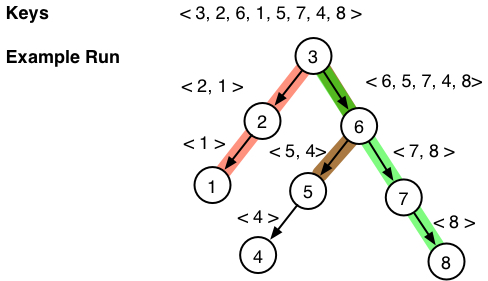
\includegraphics[width=4in]{randomized/select-example}
\end{center}
\end{example}
\end{figure}


Let's analyze the work and span of the randomized algorithm where we
pick pivots uniformly randomly.  
%
Let $n = |a|$ and define
$X(n)= \max\{|\ell|, |r|\}/|a|$, which
is the fractional size of the larger side.  Notice that $X$ is an
upper bound on the fractional size of the side the algorithm actually
recurs into.  Now since lines 3 and 4 are simply two \cd{filter}
calls, we have the following recurrences:
\begin{align*}
  \begin{array}{l c l c l}
    W(n) &\leq&  W(X(n) \cdot n) &+& O(n)\\[0.2em]
    S(n) &\leq&  S(X(n) \cdot n) &+& O(\log n)\\
  \end{array}
\end{align*}

Let's first look at the work recurrence. Specifically, we are
interested in $\expct{W(n)}$.  First, let's try to get a sense of what
happens in expectation.

The key quantity in bounding th expectation is bounding  $\expct{X(n)}$. 
%
To this end, let's none first that all pivots are equally likely.
%
We can thus draw the following plot of the size of $\ell$ and size of
$r$ as a function of where the pivot belongs in the sorted order of
$a$.
\begin{center}
  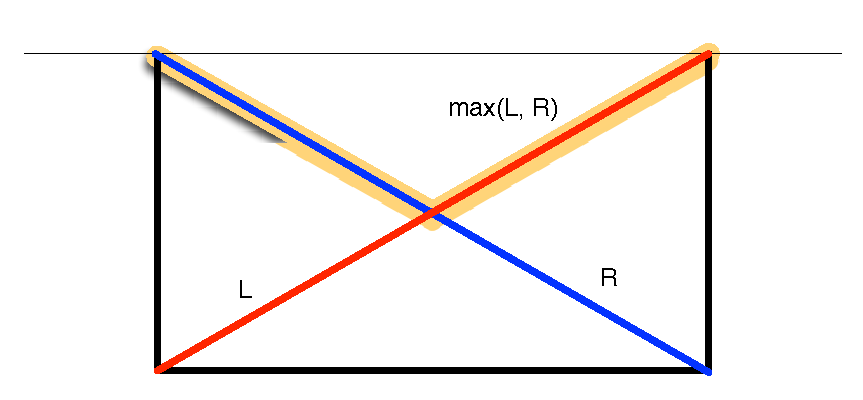
\includegraphics[scale=.6]{randomized/max-random}
\end{center}
%
If the pivot is at the start then $\ell$ is empty and $|r| =|a|-1$,
and if the pivot is at the end then $r$ is empty and $|\ell|=|a|-1$.
%
Since the probability that we land on a point on the $x$ axis is
$1/n$, we can write the expectation for $X(n)$ as
\begin{align*}
  \expct{X(n)} = \frac{1}{n} \sum_{i=0}^{n-1} \frac{\max\{i, n-i-1\}}{n} \leq \frac{1}{n} \sum_{j=n/2}^{n-1} \frac{2}{n}\cdot j \leq \frac{3}{4}
\end{align*}
(Recall that $\sum_{i=x}^y i = \frac12(x+y)(y - x + 1)$.)

%\myp{Aside:} This is a counterexample showing that $\expct{\max\{X,
%  Y\}} \neq \max\{\expct{X},\expct{Y}\}$.

This calculation tells us that in expectation, $X(n)$ is a constant
fraction smaller than $1$, so intuitively in calculating the work we
should have a nice geometrically decreasing sum that adds up to
$O(n)$.  
%
It is not quite so simple, however, since the constant
fraction is only in expectation.
%
It could also be we are unlucky for a few
contraction steps and the sequences size hardly goes down at all.  
%
We will cover other algorithms on graphs that have the same property,
i.e. that the size goes down by an expected constant factor on each
contraction step.  
%
The following theorem shows that even if we are unlucky on some steps,
the expected size will indeed go down geometrically.  Together with
the linearity of expectations this will allow us to bound the work.
%
Note that the proof of this theorem would have been relatively easy if
the successive choices made by the algorithm were independent but they
are not, because the size to the algorithm at each recursive call
depends on prior choices of pivots.
%

\begin{theorem}
\label{thm:random::contract}
Starting with size $n$, the expected size of $a$ in algorithm
\ksmall{} after
$d$ recursive calls is $\left(\frac{3}{4}\right)^d n$.  
\end{theorem}

\begin{proof}
The proof is by induction on the depth of the recursion~$d$. 
%
In the base case, $d = 0$ and the lemma holds trivially.
%
For the inductive case assume that the lemma holds for some $d  \ge 0$.
%
Consider now the $(d+1)^{th}$ recursive call.
%
Let $Y_d$ be the random variable denoting the size of the input to the
$d^{th}$ recursive call and let $Z$ the pivot chosen at the
$d^{th}$ call.
%
For any value of $y$ and $z$, let $f(y,z)$ be the fraction of the
input reduced by the choice of the pivot at position $z$ for an input of size
$y$. 
%
We can write the expectation for the input size at $(d+1)^{st}$ call
as 
\[
\begin{array}{lll}
E[Y_{d+1}] 
& = & \sum_{y,z}{y f(y,z) \pmf{Y,Z}(y,z)} 
\\
& = & \sum_{y}{\sum_{z}{y f(y,z) \pmf{Y}(y) \pmf{Z \given Y}(z \given y)}} 
\\
& = & \sum_{y}{y \pmf{Y}(y) \sum_{z}{f(y,z) \pmf{Z \given Y}(z \given y)}} 
\\
& \le & \sum_{y}{y \pmf{Y}(y) \expct{X(y)}}.
\\
& \le & \frac34 \sum_{y}{y \pmf{Y}(y)}.
\\
&\le & \frac34 \expct{Y_d}.
\end{array}
\]  

Note that we have used the bound 
\[
\expct{X(y)} = \sum_{z}{f(y,z) \pmf{Z \given Y}(z \given y)} \le \frac34,
\]
which we established above.


We thus conclude that $\expct{Y_{d+1}} = \frac34 \expct{Y_d}$, which
this trivially solves to the bound given in the theorem, since at
$d=0$ the input size is $n$.
\end{proof}

%%%% This proof is not careful about the dependency between  
%%%% random variables.
% \begin{theorem}
% \label{the:contract}
% Starting with size $n$, the expected size of $a$ in algorithm
% \ksmall{} after
% $i$ recursive calls is $\left(\frac{3}{4}\right)^i n$.  
% \end{theorem}
% %% \begin{proof}
% %% Let $Y_i$ be the random variable representing the size of the result
% %% after step (recursive call) $i$, and let $X_i$ be the random variable
% %% representing the fraction of elements that are kept on the $i^{th}$
% %% step, giving $Y_i = n \prod_{j=1}^iX_j$.  Since we pick the pivot
% %% independently on each step, the $X_j$ are independent, allowing us to
% %% take advantage of the fact that with independence the product of
% %% expectations of random variables is equal to the expectation of their
% %% products.  This gives:

% %% \[\expct{Y_i} = \expct{n \prod_{j=1}^i X_j} = n \prod_{j=1}^i
% %%   \expct{X_j} \leq \left(\frac{3}{4}\right)^i n\]
% %% \end{proof}

The work at each level of the recursive calls is linear in the size of
the input and thus can be written as $W_{\cd{select}}(n) \leq k_1n + k_2$, where $n$ is the input size.
%
Since at least one element, the pivot, is taken out of the input for
the recursive call at each level, there are at most $n$ levels of
recursion, and thus, we can bound the expected work as
\begin{eqnarray*}
\expct{W_{\ksmall}(n)}
& \leq & \sum_{i=0}^n (k_1 \expct{Y_i} + k_2) \\
\expct{W_{\ksmall}(n)}
& \leq & \sum_{i=0}^n (k_1 n \left(\frac{3}{4}\right)^i + k_2) \\
& \leq & k_1 n \left(\sum_{i=0}^n \left(\frac{3}{4}\right)^i\right) + k_2 n \\
& \leq & 4 k_1 n + k_2 n\\
& \in & O(n).
\end{eqnarray*}

\paragraph{Expected Span.}
We can bound the span of the algorithm by $O(n\lg{n})$ trivially
in the worst case, but we expect the average span to be a lot better
because chances of picking a poor pivot over and over again, which
would be required for the linear span is unlikely.
%
To bound the span in the expected case, we shall use
\thmref{random::contract} to bound the number of levels taken by
\ksmall{} more tightly using a high probability bound.
%

Consider depth $d = 10 \lg n$.
%
At this depth, the expected size upper bounded by
$n\left(\frac{3}{4}\right)^{10 \lg n}$.
%
With a little math this is equal to $n \times n^{-10 \lg (4/3)}
\approx n^{-3.15}$.
%
Now, by Markov's inequality, if the expected size is at most
$n^{-3.15}$ then the probability of having size at least $1$ is
bounded by
\[ 
\prob{Y_{10\lg n} \geq 1} \leq E[Y_{10\lg n}]/1 = n^{-3.15}. 
\]
In applying Markov's inequality, we choose $1$, because we know that
the algorithm terminates for that input size.
%
By increasing the constant factor from $10$ to $20$ would decrease the
probability to $n^{-7.15}$, which is extremely unlikely: for $n =
10^6$ this is $10^{-42}$.  
%
We have therefore shown that the number of steps is $O(\log n)$ with
high probability.  
%
Each step has span $O(\log n)$ so the overall span is $O(\log^2 n)$
with high probability.

Using the high probability bound, we can bound the expected span by
using the total expectation theorem.
%
For brevity let the random variable $Y$ be defined as $Y = Y_{10\lg n}$,
%
\[
\begin{array}{lll}
\expct{S} & = & \sum_{y}\pmf{Y}(y) \expct{S \given Y = y}.
\\
& = & 
\sum_{y \le 1}{\pmf{Y}(y) \expct{S \given Y = y}}
 + 
\sum_{y >1}{\pmf{Y}(y) \expct{S \given Y = y}}
\\
& \le & 
(1 - n^{-3.5}) O(\lg^2{n}) 
 + 
n^{-3.5} O(n)
\\
& = &
O(\lg^2{n}). 
\end{array}
\]

The expected bound follows by the fact that with high probability the
depth of the recursive calls is $O(\lg{n})$ and that each
recursive call has $O(\lg{n})$ span, because it requires a
sequences \cd{filter}.
%
The span for the case when the span is not greater that $10\lg{n}$
contributes only a constant value to the expectation as long as it is
a polynomial that is less that $n^{3.5}$.

In summary, we have shown than the \ksmall{} algorithm on input of
size $n$ does $O(n)$ work in expectation and has $O(\log^2 n)$ span
with high probability.  
%
As mentioned at the start of the chapter, we will typically be
analyzing work using expectation and span using high probability.

\begin{notesonly}
%% Please do not delete this analysis.  It is helpful.
\paragraph{Alternative Analysis.}

Let $Z_n$ denote the random variable denoting the size of the maximum
of the two subsequences computed by splitting inpet sequence of size
$n$ by the pivot.
%
We can see that $\prob{Z(n) \le \frac34 n} \ge \frac12$, because
choosing any one of the elements between rank $\frac{n}{4}$ and
$\frac{3n}{4}$ yield such a fairly balanced partition.
%

Using total expectation theorem, we can write the expected work of the
algorithm by conditioning on the random variable $Z$.
\[
\expct{W(n)} = \sum_{i = z}^{n}{\prob{Z(n) = z} \cdot \expct{W(n}  \given n = z} + O(n).
\]
We can bound this sum as follows
\[
\begin{array}{lll}
\expct{W(n)} 
& = & 
\sum_{i = z}^{n}{\prob{Z(n) = z} \cdot \expct{W(n}  \given n = z} + O(n).
\\
& = & 
\sum_{i = z}^{n}{\prob{Z(n) = z} \cdot \expct{W(z}} + O(n).
\\
& \le & 
\prob{Z(n) \le \frac34 n} \cdot \expct{W(\frac34 n} 
+ 
\prob{Z(n) > \frac34 n} \cdot \expct{W(n)}
+
O(n)
\\
& \le & \frac12 \expct{W(\frac34 n)} +  \frac12 \expct{W(n)} + O(n).
\end{array}
\]

We now have the following recurrence
\[
\expct{W(n)} 
\le 
\frac12 \expct{W(\frac34 n)} +  \frac12 \expct{W(n)} + O(n),
\]
which can be simplified as 
\[
\expct{W(n)} 
\le 
\expct{W(\frac34 n)} + O(n).
\]

This solves to $O(n)$.  Exactly the same approach can be followed to
obtain the following recurrence for span
\[
\expct{W(n)} 
\le 
\expct{W(\frac34 n)} + O(\lg{n}).
\]
This solves to $O(\lg^2{n})$.
\end{notesonly}

\section{\Qsort}
Moving on to a more complex algorithm, let's analyze the work and span
of the randomized \qsort{} algorithm.
%
In later chapters we will see that the analysis of \qsort{} presented
here is is effectively identical to the analysis of a certain type of
balanced tree called Treaps.  
%
It is also the same as the analysis of ``unbalanced'' binary search
trees under random insertion.


Consider the \qsort{} algorithm given in \algref{randomized::qsort}.
In this algorithm, we intentionally leave the pivot-choosing step
unspecified because the property we are discussing holds regardless of
the choice of the pivot.

\begin{figure}
\begin{algorithm}[Quicksort]~
\label{alg:randomized::qsort}
\begin{lstlisting}
quicksort $a$ =
if $|a| = 0$ then $a$
else 
  let
    $p = \ctext{pick a pivot from } a$ @\label{line:randomized::qsort-rk}@
    $a_1 = \cseqf{x \in a}{x < p}$
    $a_2 = \cseqf{x \in a}{x = p}$
    $a_3 = \cseqf{x \in a}{x > p}$
    $(s_1,s_3)$ = (sort $a_1$ || sort $a_3$)
  in
    $s_1$ ++ $a_2$ ++ $s_3$
  end
\end{lstlisting}
\end{algorithm}
\end{figure}

\begin{question}
Is there parallelism in \qsort{}?
\end{question}

There is plenty of parallelism in this version \qsort{}.
%
There is both parallelism due to the two recursive calls and in the
fact that the filters for selecting elements greater, equal, and less
than the pivot can be parallel.


Note that each call to \qsort{} either makes no recursive calls (the
base case) or two recursive calls.  The call tree is therefore binary.
We will often find it convenient to map the run of a \qsort{} to a
binary-search tree (BST) representing the recursive calls along with
the pivots chosen.  
%
We will sometimes refer to this tree as the {\em call tree} or
\defn{pivot tree}.
%
We will use this call-tree representation to reason about the
properties of \qsort{}, e.g., the comparisons performed, its span.  An
example is shown in \exref{randomized::qsort}.

\begin{figure}
\begin{example}
\label{ex:randomized::qsort}
An example run of \qsort{} along with its pivot tree.
\begin{center}
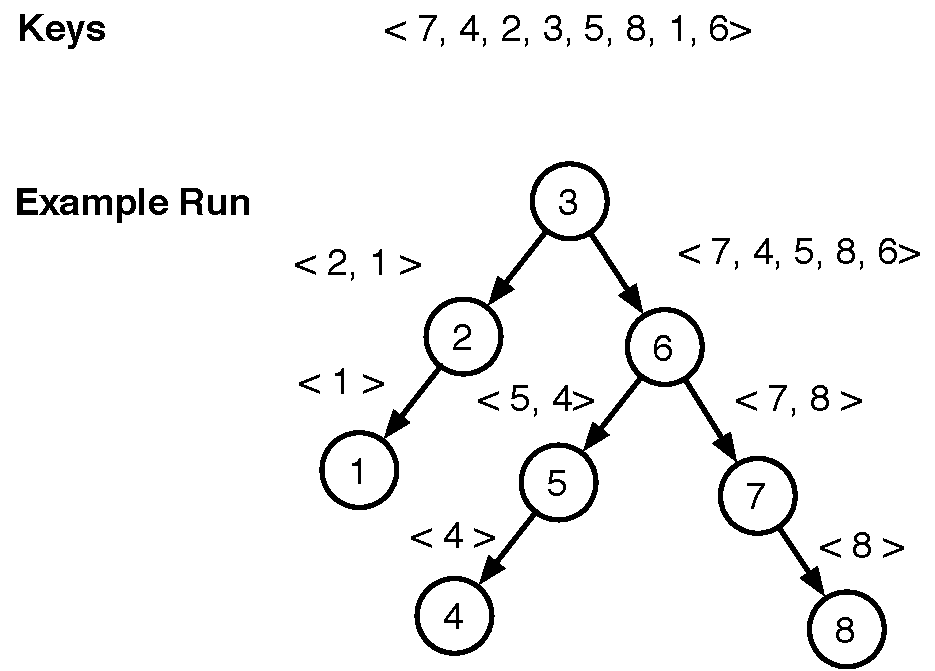
\includegraphics[width=4in]{randomized/qsort-bst-example}
\end{center}
\end{example}
\end{figure}


%% \begin{example}
%% An example call tree, which is a binary-search-tree, illustrated. 
%% \begin{center}
%% 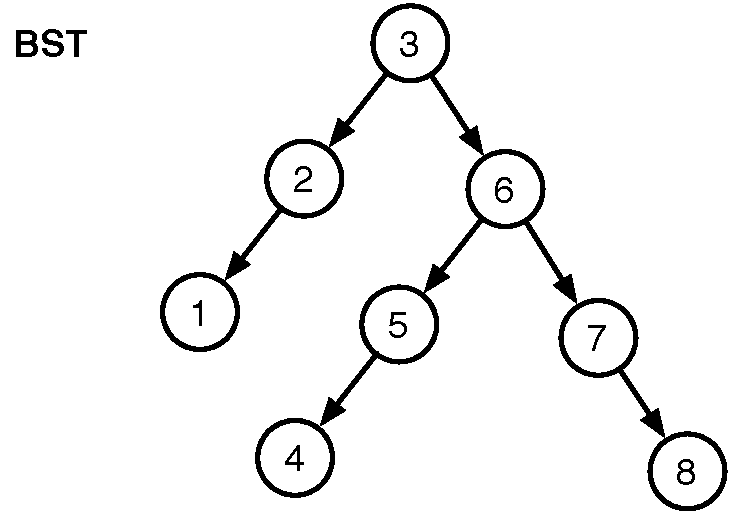
\includegraphics[width=3in]{randomized/qsort-bst-1}
%% \end{center}
%% \end{example}

Let's consider some strategies for picking a pivot.   
\begin{itemize}
\item \textbf{Always pick the first element:} If the sequence is sorted
  in increasing order, then picking the first element is the same as
  picking the smallest element.  We end up with a lopsided recursion
  tree of depth $n$.  The total work is $O(n^2)$ since $n-i$ keys will
  remain at level $i$ and hence we will do $n-i-1$ comparisons at that
  level for a total of $\sum_{i=0}^{n-1} (n-i-1)$.  Similarly, if the
  sequence is sorted in decreasing order, we will end up with a
  recursion tree that is lopsided in the other direction.  In
  practice, it is not uncommon for a sort function input to be a
  sequence that is already sorted or nearly sorted.

\item \textbf{Pick the median of three elements:} Another strategy is to
  take the first, middle, and the last elements and pick the median of
  them.  For sorted lists the split is even, so each side contains
  half of the original size and the depth of the tree is $O(\log n)$.
  Although this strategy avoids the pitfall with sorted sequences, it
  is still possible to be unlucky, and in the worst-case the costs and
  tree depth are the same as the first strategy.  This is the strategy
  used by many library implementations of \qsort{}.  Can you think of
  a way to slow down a \qsort{} implementation that uses this
  strategy by picking an adversarial input?

\item \textbf{Pick an element randomly:} It is not immediately clear
  what the depth of this is, but intuitively, when we choose a random
  pivot, the size of each side is not far from $n/2$ in expectation.
  This doesn't give us a proof but it gives us hope that this strategy
  will result in a tree of depth $O(\log n)$ in expectation or with
  high probability.  Indeed, picking a random pivot gives us expected
  $O(n \log n)$ work and $O(\log^2 n)$ span for \qsort{} and an
  expected $O(\log n)$-depth tree, as we will show.
\end{itemize}



% The next question to ask is: \emph{Is this a good BST?}  A reasonable question
% to start with is to find out how deep this tree is.  If the tree is about
% $O(\log n)$ deep, then it must be a pretty good tree.  So then, what determines
% the depth of this tree?  As we discussed already, the depth of the BST is the
% same as the depth of the recursion tree for \qsort{}, so the choice of pivots
% determines the depth of the BST.  Let's consider some strategies for picking a
% pivot:
% \begin{itemize}
% \item \emph{Always pick the smallest element:} We end up with a lopsided
%   tree. In fact, each node only has a right child (and no left child). This is a
%   linked-list.
% \item \emph{Always pick the largest element:} Again, we end up with a lopsided
%   tree, where each node has a left child only (no left child). This is, again, a
%   linked-list.
% \item \emph{Pick the median element:} The split is even, so each side contains
%   half of the original size and the depth of the tree is $O(\log n)$.

% \item \emph{Pick an element randomly:} It is not immediately clear what the
%   depth of this is, but intuitively, when we choose a random pivot, the size of
%   each side is about $n/2$ in expectation.  This doesn't give us a proof but it
%   gives us hopes that this strategy will result in a tree of depth $O(\log n)$
%   in expectation.  Indeed, picking a random pivot gives us expected $O(\log
%   n)$-depth tree.
% \end{itemize}

\section*{Analysis of \Qsort{}}

To develop some intuition for the span analysis, let's consider the
probability that we split the input sequence more or less evenly.
%
\begin{question}
What is the probability that $X(n)$ is at most $3n/4$? 
\end{question}
%
If we select a pivot that is greater than $t_{n/4}$ and less than
$t_{3n/4}$ then $X(n)$ is at most $3n/4$.  Since all keys are equally
  likely to be selected as a pivot this probability is $\frac{3n/4 - n/4}{n} =
  1/2$.  The figure below illustrates this.

\begin{center}
\centering
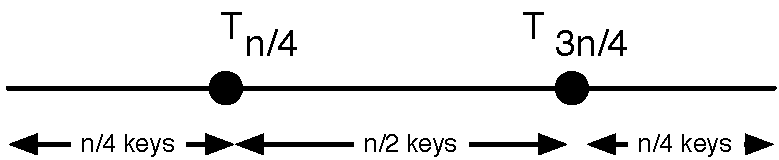
\includegraphics[width=4in]{randomized/qsort-span-intuition}
\end{center}

\begin{question}
What does this say about what the span of $\cdm{\qsort{}}$ may be? 
\end{question}

This observations implies that at each level of the call tree (every
time a new pivot is selected), the size of the input to both calls
decrease by a constant fraction (of $3/4$).
%
At every two levels, the probability that the input size decreases by
$3/4$ is the probability that it decreases at either step, which is at
least $1-\frac12 \cdot \frac12 = \frac34$, etc.
%
More generally, after $m$ such steps, the probability that the input
size decreases by a factor of $3/4$ is $1 - \frac{1}{2}^m$.
%
Thus the probability that the input size decreases by a factor of
$3/4$ approaches $1$ quickly.  For example if $m = 10$ then this
probability is $0.999$.
%
Thus we can conclude that \qsort{} behaves like a balanced divide and
conquer algorithm and it should complete after $c\log{n}$ levels for
some constant $c$.


We now make this intuition more precise.  There are many methods of
analysis that we can use.  In the rest of this section, we consider
one in detail, which is based on counting, and outline another, which
is based establishing a recurrence, which can then be solved.
%

For the analysis, we assume a priority-based selection technique for
pivots.
%
At the start of the algorithm, we assign each key a random priority
uniformly at random from the real interval $[0, 1]$ such that each key
has a unique priority.  
%
We then pick in \lineref{randomized::qsort-rk}
the key with the highest priority.  Notice that once the priorities
are decided, the algorithm is completely deterministic.
%
In addition, we assume a version of quicksort that compares the pivot
$p$ to each key in $S$ once (instead of 3 times, once to generate each
of $a_1$, $a_2$, and $a_3$).
%
\begin{exercise}
  Rewrite the quicksort algorithm so to use the comparison once when
  comparing the pivot with each key at a recursive call.
\end{exercise}
%


\begin{example}

\Qsort{} with priorities and its call tree, which is a binary-search-tree, illustrated. 

\begin{center}
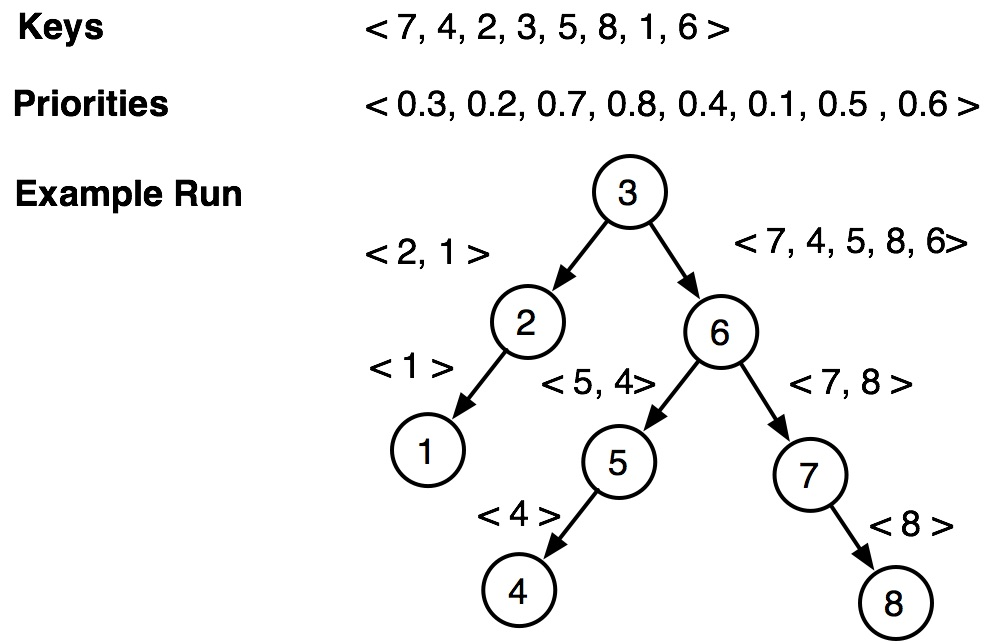
\includegraphics[width=4in]{randomized/qsort-bst-example-with-p}
\end{center}

\end{example}

\begin{exercise}
Convince yourself that the two
presentations of randomized \qsort{} are fully equivalent (modulo the
technical details about how we might store the priority values).
\end{exercise}

Before we get to the analysis, let's observe some properties of
\qsort{}.  For these observations, it might be helpful to consider the
example shown above.  
\begin{itemize}
\item In \qsort{}, a comparison always involves a
pivot and another key.  

\item Since, the pivot is not sent as part of the input to a recursive
  call, a key is selected to be a pivot at most once.

\item Each key is selected to be pivot.
 
\end{itemize}

Based on these observations, we conclude that each pair of keys is
compared at most once.
%
\footnote{We need only the first two observations to establish this
  conclusion.}
%




%% \begin{notesonly}

%% \begin{question}
%% Can you tell which keys are compared by looking at just the call tree? 
%% \end{question}


%% Following the discussion above, we can see that a key is compared with
%% all its ancestors in the call tree, and all its descendants in the
%% call tree, once for each ancestor and descendant.
%% %
%% \begin{question}
%%   Let $x$ and $z$ two keys such that $x < z$.  Suppose that a key $x <
%%   y < z$ is selected as a pivot before either $x$ or $z$ is selected.
%%   Are $x$ and $z$ compared?
%% \end{question}
%% %
%% When the algorithm selects a key say $y$ in between two keys say $x$
%% and $z$ as a pivot, it sends the two keys to two separate subtrees.
%% The two keys $x$ and $z$ separated in this way are never compared
%% again.
%% \begin{question}
%% Suppose that the keys $x$ and $y$  are adjacent in the sorted order,
%%   how many times are they compared? 
%% \end{question}
%% Adjacent keys are compared exactly once.  This is the case because
%% there is no key that will ever separate them.  
%% \begin{question}
%% Would it be possible to modify \qsort{} so that it never compares
%% adjacent keys?
%% \end{question}
%% Indeed adjacent keys must be compared by any sorting algorithm since
%% otherwise it would be impossible to tell which one appears first in
%% the output.

%% \begin{question}
%%   Based on these observations, can you bound the number of comparisons
%%   performed by \qsort{} in terms of the comparisons between keys.
%% \end{question}
%% \end{notesonly}

\paragraph*{Expected work for \Qsort{}.}
We are now ready to analyze the expected work of randomized \qsort{}
by counting how many comparisons $\cdm{\qsort{}}$ it makes in
expectation.  
%
We introduce a random variable
\begin{equation*}
 Y(n) ~~~=~~~\mbox{number of comparisons \cdm{\qsort{}} makes on input
   of size}~n,
\end{equation*}
and we are interested in finding an upper bound on $\expct{Y(n)}$.  In
particular we will show it is in $O(n \log n)$.
%
 $\expct{Y(n)}$ will not depend on the order of the input sequence.

Consider the final sorted order of the keys $t = \cd{sort}(a)$
%
and
%
let $p_i$ be the priority we chose for the element $t_i$. 
%
Consider two positions $i, j \in \{1, \dots, n\}$ in the sequence $t$
and define following random variable
\begin{eqnarray*}
X_{ij} 
%
& = &
%
\left\{\begin{array}{ll}
1 & \mbox{if $t_i$ and $t_j$ are compared by \qsort{}}\\
0 & \mbox{otherwise}
\end{array}\right.
\end{eqnarray*}
%
Since in any run of \qsort{}, each pair of keys is compared at most
once, $Y(n)$ is equal to the sum of all $X_{ij}$'s, i.e.,
\[
Y(n) \;\; \leq \;\; \sum_{i=1}^n \sum_{j=i+1}^n X_{ij}
\]
Note that we only need to consider the case that $i < j$ since we only
want to count each comparison once.
By linearity of expectation, we have
\[
 \expct{Y(n)} \leq \sum_{i=1}^n \sum_{j=i+1}^n \expct{X_{ij}}
\]
%
Since each $X_{ij}$ is an indicator random variable,
$\expct{X_{ij}} = \prob{X_{ij} = 1}$.  


\begin{figure}
\centering
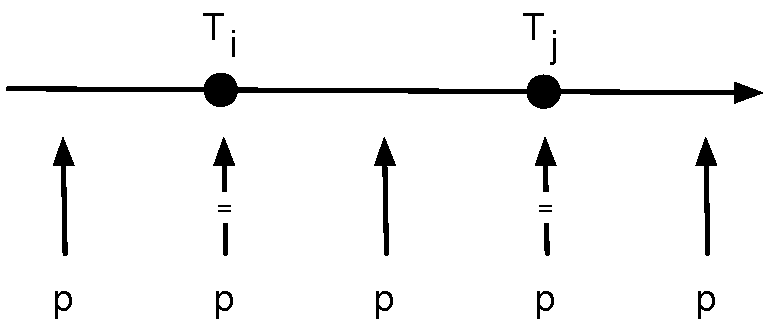
\includegraphics[width=3in]{randomized/qsort-cases}
\caption{The possible relationships between the selected pivot $p$, $t_i$ and $t_j$ illustrated.}
\label{fig:lec18::cases}
\end{figure}


To compute the probability that $t_i$ and $t_j$ are compared (i.e.,
$\prob{X_{ij}=1}$), 
%
let's take a closer look at the \qsort{} algorithm to gather some
intuitions.  
%
Notice that the first recursive call takes as its pivot $p$ the
element with highest priority.  
%
Then, it splits the sequence into two parts, one with keys larger than
$p$ and the other with keys smaller than $p$.  For each of these
parts, we run $\cdm{\qsort{}}$ recursively; therefore, inside it, the
algorithm will pick the highest priority element as the pivot, which
is then used to split the sequence further.

For any one call to $\cdm{\qsort{}}$ there are three possibilities
(illustrated in Figure~\ref{fig:lec18::cases})
for $X_{ij}$, where $i < j$:
\begin{itemize}
\item The pivot (highest priority element) is either $t_i$ or $t_j$,
  in which case $t_i$ and $t_j$ are compared and $X_{ij} = 1$.
\item The pivot is element between $t_i$ and $t_j$, in which case
  $t_i$ is in $a_1$ and $t_j$ is in $a_3$ and $t_i$ and $t_j$ will
  never be compared and $X_{ij} = 0$.
\item The pivot is less than $t_i$ or greater than $t_j$.  Then 
  $t_i$ and $t_j$ are either both in $a_1$ or both in $a_3$,
  respectively.  Whether $t_i$ and $t_j$ are compared will be
  determined in some later recursive call to $\cdm{\qsort{}}$.
\end{itemize}

With this intuition in mind, we can establish the following claim.
\begin{claim}
  For $i < j$, $t_i$ and $t_j$ are compared if and only if $p_i$ or $p_j$ has the highest
  priority among $\{p_i, p_{i+1},\dots, p_j\}$.
\end{claim}
\begin{proof}
Assume first that $t_i$ ($t_j$) has the highest priority.  In this
case, all the elements in the subsequence $t_i \ldots t_j$ will move
together in the call tree until $t_i$ ($t_j$) is selected as pivot.
%
When it is selected as pivot, $t_i$ and $t_j$ will be compared. 
%
This proves the first half of the claim.

For the second half, assume that $t_i$ and $t_j$ are compared.  For
the purposes of contradiction, assume that there is a key $t_k$, $i <
k < j$ with a higher priority between them.  In any collection of keys
that include $t_i$ and $t_j$, $t_k$ will become a pivot before either
of them.  Since $t_i \leq t_k \leq t_j$ it will separate $t_i$ and
$t_j$ into different buckets, so they are never compared.  This is a
contradiction; thus we conclude there is no such $t_k$.
\end{proof}

Therefore, for $t_i$ and $t_j$ to be compared, $p_i$ or $p_j$ has to
be bigger than all the priorities in between.  
%
Since there are $j-i+1$ possible keys in between (including both $i$
and $j$) and each has equal probability of being the highest, the
probability that either $i$ or $j$ is the highest is $2/(j-i+1)$.
%
Therefore,
%
\begin{align*}
  \expct{X_{ij}} &= \prob{X_{ij} = 1} \\
  &= \prob{p_i \text{ or } p_j \text{ is the maximum among } \{p_i, \dots, p_j\}} \\
  &= \frac{2}{j - i + 1}.
\end{align*}

% More formally, we also consider the third case when the pivot is less than $T_i$
% or greater the $T_j$.  In this case, some later recursive call to \cd{\qsort{}} will
% determine whether the two are compared.  Let $B_r$ be event that the $r^{th}$
% recursive call is the first call where the highest priority is among $\{p_i, p_{i+1},\dots,
% p_j\}$. Notice that the events $B_1, B_2, \ldots $ are disjoint and
% with probability 1 one of the events will eventually occur.  

% Therefore,
% \begin{align*}
%   \expct{X_{ij}} &= \sum_r \prob{B_r} \expct{X_{ij} = 1 \;|\; B_r} \\
%   &= \sum_r \prob{B_r} \prob{p_i \text{ or } p_j \text{ is the maximum } |\; B_r} \\
%   &= \sum_r \prob{B_r} \frac{2}{j - i + 1} \\
%   &= \frac{2}{j - i + 1}\sum_r \prob{B_r} \\
%   &= \frac{2}{j - i + 1}.
% \end{align*}


\begin{question}
What does this bound tell us about the likelihood of keys being compared? 
\end{question}

The bound indicates that the closer two keys are in the sorted order
($t$) the more likely it is that they are compared.  For example, the
keys $t_i$ is compared to $t_{i+1}$ with probability~1. It is easy to
understand why if we consider the corresponding pivot tree. 
%
One of $t_i$ and $t_{i+1}$ must be an ancestor of the other in the
pivot tree: there is no other element that could be the root of a
subtree that has $t_i$ in its left subtree and $t_{i+1}$ in its right
subtree.
%
Regardless, $t_i$ and $t_{i+1}$ will be compared.

If we consider $t_{i}$ and $t_{i+2}$ there could be such an element,
namely $t_{i+1}$, which could have $t_i$ in its left subtree and
$t_{i+2}$ in its right subtree. That is, with probability $1/3$,
$t_{i+1}$ has the highest probability of the three and $t_i$ is not
compared to $t_{i+2}$, and with probability $2/3$ one of $t_i$ and
$t_{i+2}$ has the highest probability and, the two are compared.  In
general, the probability of two elements being compared is inversely
proportional to the number of elements between them when sorted.  The
further apart the less likely they will be compared.  Analogously, the
further apart the less likely one will be the ancestor of the other in
the related pivot tree.

Hence, the expected number of comparisons made in randomized $\cdm{\qsort{}}$ is
\begin{align*}
  \expct{Y(n)} &\leq \sum_{i=1}^{n-1} \sum_{j=i+1}^n \expct{X_{ij}}
\\
  &= \sum_{i=1}^{n-1}  \sum_{j=i+1}^n \frac{2}{j-i+1}
\\
  &= \sum_{i=1}^{n-1}  \sum_{k=2}^{n-i+1} \frac{2}{k} 
\\
  & \leq 2n \sum_{i=1}^{n-1}  H_n 
\\
  &= 2n H_n \in O(n\log n).
\end{align*}
Note that in the derivation of the asymptotic bound, we used the fact
that $H_n = \ln{n} + O(1)$.

Indirectly, we have also shown that the average work for the basic
deterministic $\cdm{\qsort{}}$ (always pick the first element) is also $O(n
\log n)$.  Just shuffle the data randomly and then apply the basic
$\cdm{\qsort{}}$ algorithm.  Since shuffling the input randomly results in the
same input as picking random priorities and then reordering the data
so that the priorities are in decreasing order, the basic $\cdm{\qsort{}}$ on
that shuffled input does the same operations as randomized $\cdm{\qsort{}}$
on the input in the original order.  Thus, if we averaged over all
permutations of the input the work for the basic $\cdm{\qsort{}}$ is $O(n
\log n)$ on average.


\paragraph{Expected span of \Qsort{}.}
We now analyze the span of $\cdm{\qsort{}}$.  All we really need to
calculate is the depth of the pivot tree, since each level of the tree
has span $O(\log n)$---needed for the filter.  We argue that the depth
of the pivot tree is $O(\log n)$ by relating it to the number of
contraction steps of the randomized \cd{select} we considered
in \secref{sec:randomized::select}.  
%
We refer to the $i^{th}$ node of
the pivot tree as the node corresponding to the $i^{th}$ smallest key.
This is also the $i^{th}$ node in an in-order traversal.

\begin{claim}
The path from the root to the $i^{th}$ node of the pivot tree is the
same as the steps of \cd{select} on $k = i$.  That is to the
say that the distribution of pivots selected along the path and the
sizes of each problem is identical.
\end{claim}

The reason this is true, is that \cd{select} is the same as
\cd{quicksort} except that it only goes down one of the two recursive
branches---the branch that contains the $k^{th}$ key.
%
Recall that for \cd{select}, we showed that the length of the
path is more than $10 \lg n$ with probability at most $1/n^{3.15}$.
%
This means that the length of any path being longer that $10\lg{n}$ is
tiny.
%
\begin{question}
Can we thus say that there can be no long paths.
\end{question}
This does not suffice to conclude, however, that there are no paths
longer than $10\lg{n}$, because there are many paths in the pivot
tree, and because we only need one to be long to impact the span.
%
Luckily, we don't have too many paths to begin with.
%
We can take advantage of this property by using the union bound,
%
which
%
says that the probability of the union of a collection of events is at
most the sum of the probabilities of the events.
%
To apply the union bound, consider the event that the depth of a node
along a path is larger $10 \lg n$, which is $1/n^{3.5}$.
%
The total probability that any of the $n$ leaves have depth larger
than $10 \lg n$ is
\[
\prob{\mbox{depth of \qsort{} pivot tree} > 10 \lg n} 
\leq 
\frac{n}{n^{3.15}} = \frac{1}{n^{2.15}}.
\]
%
We thus have our high probability bound on the depth of the pivot tree.

The overall span of randomized $\cdm{\qsort{}}$ is therefore $O(\log^2 n)$
with high probability.
%
As in \cd{select}, we can establish an expected bound by using the
total expectation theorem.
%
We leave this as an exercise to the reader.

\begin{notesonly}
Using the high probability bound, we can bound the expected span by
using the total expectation theorem.
%
For brevity let the random variable $Y$ be defined as $Y = Y_{10\lg n}$,
%
\[
\begin{array}{lll}
\expct{S} & = & \sum_{y}\pmf{Y}(y) \expct{S \given Y = y}.
\\
& = & 
\sum_{y \le 1}{\pmf{Y}(y) \expct{S \given Y = y}}
 + 
\sum_{y >1}{\pmf{Y}(y) \expct{S \given Y = y}}
\\
& \le & 
(1 - n^{-2.5}) O(\lg^2{n}) 
 + 
n^{-2.5} O(n^2)
\\
& = &
O(\lg^2{n}). 
\end{array}
\]

\end{notesonly}

\paragraph{Alternative Analysis.}

Another way to analyze the work of $\cdm{\qsort{}}$ is to write a recurrence
for the expected work (number of comparisons) directly.  This is the
approach taken by Tony Hoare in his original paper.  For simplicity we
assume there are no equal keys (equal keys just reduce the cost).  The
recurrence for the number of comparisons $Y(n)$ done by $\cdm{\qsort{}}$ is
then:
\begin{eqnarray*}
Y(n) & = & Y(X(n)) + Y(n-X(n)-1) + n -1
\end{eqnarray*}
where the random variable $Y(n)$ is the size of the set $a_1$ (we
use $X(n)$ instead of $Y_n$ to avoid double subscripts).  We can now write
an equation for the expectation of $X(n)$.
\begin{eqnarray*}
\expct{Y(n)} & = & \expct{Y(X(n)) + Y(n-X(n)-1) + n -1}\\
             & = & \expct{Y(X(n))} + \expct{Y(n-X(n)-1)} + n -1\\
             & = & \frac{1}{n} \sum_{i=0}^{n-1}(\expct{Y(i)} + \expct{Y(n-i-1)}) + n -1
\end{eqnarray*}
where the last equality arises since all positions of the pivot are
equally likely, so we can just take the average over them.  
%
This can be by guessing the answer and using substitution.  It gives
the same result as our previous method.  We leave this as exercise.


We can use a similar strategy to analyze span.
%
Recall that in randomized $\cdm{\qsort{}}$, at each recursive call, we
partition the input sequence $a$ of length $n$ into three subsequences
$a_1$, $a_2$, and $a_3$, such that elements in the subsequences are
less than, equal, and greater than the pivot, respectfully.  
%
Let the random variable $X(n)
= \max\{|a_1|, |a_2|\}$, which is the size of larger subsequence. 
%
The span of $\cdm{\qsort{}}$ is determined by the sizes of these larger
subsequences. For ease of analysis, we will assume that $|a_2| = 0$, as
more equal elements will only decrease the span. As this partitioning
uses \cd{filter} we have the following recurrence for span for input
size $n$

\[ 
S(n) = S(X(n)) + O(\log n). 
\]

For the analysis, we shall condition the span on the random variable
denoting the size of the maximum half and apply the total expectation
theorem.
%%
%% As we did for \sml{SmallestK}, we will bound $E[a_n]$ by considering
%% the $\prob{Y_n \leq 3n/4}$ and $\prob{Y_n > 3n/4}$ and use the maximum
%% sizes in the recurrence to upper bound $\expct{a_n}$. Now, the
%% $\prob{Y_n \leq 3n/4} = 1/2$, since half of the randomly chosen pivots
%% results in the larger partition to be at most $3n/4$ elements: Any
%% pivot in the range $T_{n/4}$ to $T_{3n/4}$ will do, where $T$ is the
%% sorted input sequence.

\[
\expct{S(n)} = \sum_{m=n/2}^{n}{\prob{X(n)=m} \cdot \expct{S(n) \given (X(n)=m)}}.
\]

The rest is algebra
\begin{align*}
\expct{a_n} 
&=  \sum_{m=n/2}^{n}{\prob{M(n)=m} \cdot \expct{S(n) \given (M(n)=m)}}
\\
&\leq 
\prob{X(n) \leq \frac{3n}{4}} \cdot \expct{S({\frac{3n}{4}})} + 
\prob{X(n) > \frac{3n}{4}} \cdot \expct{S(n)} + c\cdot \log n
\\
&\leq \frac{1}{2} \expct{S({\frac{3n}{4}})} + \frac{1}{2} \expct{S(n)}
\\
&\implies \expct{S(n)} \leq \expct{S(\frac{3n}{4})} + 2c \log n.
\\
\end{align*}
This is a recursion in $\expct{S(\cdot)}$ and solves easily to 
 $\expct{S(n)} = O(\log^2 n)$.

% That is, with probability $1/2$ we will be
% lucky and the subproblem size will go down by at least $3n/4$ and with
% probability $1/2$ we will be unlucky and we have to start again.  In
% the end,
% the expected span is twice what it would be if we could
% guarantee partition sizes of $n/4$ and $3n/4$.


% \newcommand{\sbar}{\overline{S}}
%  Let $\sbar(n)$ denote
% $\expct{S(n)}$. As we did for \sml{SmallestK} we will bound $\sbar(n)$
% by considering the $\prob{Y_n \leq 3n/4}$ and $\prob{Y_n > 3n/4}$ and use the maximum sizes in the recurrence to upper
% bound $\expct{S(n)}$. Now, the $\prob{Y_n \leq 3n/4} = 1/2$, since
% half of the randomly chosen pivots results in the larger partition
% to be at most $3n/4$ elements: Any pivot in the range $T_{n/4}$ to
% $T_{3n/4}$ will do, where $T$ is the sorted input sequence.

% So then, by the definition of expectation, we have
% \begin{align*}
%   \sbar(n) &= \leq \sum_{i} \prob{Y_n = i } \cdot \sbar(i) + c\log n \\
%   &\leq \prob{Y_n \leq \tfrac{3n}4} \sbar(\tfrac{3n}4) + \prob{Y_n >
%     \tfrac{3n}4} \sbar(n) + c\cdot \log n\\
%   &\leq \tfrac12 \sbar(\tfrac{3n}4) + \tfrac12 \sbar(n) + c\cdot \log n\\
%   &\implies (1- \tfrac12)\sbar(n) \leq \tfrac12 \sbar(\tfrac{3n}4) + c\log n \\
%   &\implies \sbar(n) \leq \sbar(\tfrac{3n}4) + 2c \log n,
% \end{align*}
% which we know is a balanced cost tree and solves to $O(\log^2 n)$.

% That is, with probability $1/2$ we will be
% lucky and the subproblem size will go down by at least $3n/4$ and with
% probability $1/2$ we will be unlucky and we have to start again.  In
% the end,
% the expected span is twice what it would be if we could
% guarantee partition sizes of $n/4$ and $3n/4$.




\begin{remark}
\Qsort{} is one of the earliest and most famous algorithms. It was
invented and analyzed by Tony Hoare around 1960.  This was before the
big-O notation was used to analyze algorithms.  Hoare invented the
algorithm while an exchange student at Moscow State University while
studying probability under Kolmogorov---one of the most famous
researchers in probability theory.  The analysis we will cover is
different from what Hoare used in his original paper, although we will
mention how he did the analysis.  It is interesting that while
\Qsort{} is often used as an quintessential example of a recursive
algorithm, at the time, no programming language supported recursion
and Hoare spent significant space in his paper explaining how to
simulate recursion with a stack.

We note that our presentation of \qsort{} algorithm shown in
\algref{randomized::qsort} differs from Hoare's original version which
sequentially partitioned the input by using two fingers that moved
from each end and by swapping two keys whenever a key was found on the
left greater than the pivot and on the right less than the pivot.

\end{remark}

\begin{comment}

\section{Lower Bounds}

After spending time formulating a concrete problem, we might wonder how hard the
problem actually is.   In this book thus far, our focus has been on obtaining
efficient algorithms for certain problems.  For a problem $P$, we try to design
efficient algorithms to solve it.  The existence of an algorithm gives an upper
bound on the complexity of the problem $P$.  In particular, an algorithm $A$
with work (either expected or worst-case) $O(f(n))$ is a constructive proof that
$P$ can be solved provided $O(f(n))$ work.  This is essentially the upper bound
part of the question.


In this lecture, we'll turn the tables, showing that certain problems cannot be
solved more efficiently than a given bound.  This is the lower bound part of the
question.  In general, this is a harder task: To establish a lower bound, we
have to argue that \emph{no algorithm, however smart, can possibly do better
  than what we claim}; it is no longer sufficient to exhibit an algorithm $A$
and analyze its performance.

\subsection{Sorting and Merging Lower Bounds}

Before we look at lower bounds for sorting and merging, let us review the
(upper) bounds we have for various sorting algorithms we've covered:

\begin{center}
\begin{tabular}{l l l}
  \toprule
  \textbf{Algorithm} & Work & Span \\
  \midrule
  Quick Sort & $O(n\log n)$ & $O(\log^2 n)$ \\
  Merge Sort & $O(n\log n)$ & $O(\log^2 n)$ \\
  Heap Sort & $O(n \log n)$ & $O(n \log n)$ \\
  Balanced BST Sort & $O(n \log n)$ & $O(\log^2 n)$\\
  \bottomrule
\end{tabular}
\end{center}
Notice that in this table, all algorithms have $O(n \log n)$ work---and except
for heap sort, every algorithm is very parallel ($\log^2 n$ span).  Can we sort
in less than $O(n \log n)$ work?  Probably. But we'll show that
\emph{any} deterministic \emph{comparison-based}
sorting algorithm must use $\Omega(n\log n)$ comparisons to sort $n$
entries in the worst case.  In the comparison-based model, we have no domain knowledge about the
entries and the only operation we have to determine the relative order of a pair
of entries $x$ and $y$ is a comparison operation, which returns whether $x <
y$. More precisely, we'll prove the following theorem:
\begin{theorem}
  \label{thm:sorting-lb}
  For a sequence $\langle x_1, \dots, x_n \rangle$ of $n$ distinct entries,
  finding the permutation $\pi$ on $[n]$ such that $x_{\pi(1)} < x_{\pi(2)} <
  \dots < x_{\pi(n)}$ requires, in the worst case, at least $\frac{n}2\log(\frac{n}2)$
  queries to the $<$ operator.
\end{theorem}

Since each comparison takes at least constant work, this implies an $\Omega(n
\log n)$ lower bound on the work required to sort a sequence of length $n$ in
the comparison model.


What about merging? Can we merge sorted sequences faster than resorting them?
As seen in previous lectures, we can actually merge two sorted sequences in $O(m
\log (1+n/m))$ work, where $m$ is the length of the shorter of the two
sequences, and $n$ the length of the longer one.  We'll show, however, that in
the comparison-based model, we cannot hope to do better:
\begin{theorem}
  \label{thm:merging-lb}
  Merging two sorted sequences of lengths $m$ and $n$ ($m \leq n$) requires at least
  \[ m \lg(1+\tfrac{n}m)
  \]
  comparison queries in the worst case.
\end{theorem}

\subsection{Decision Trees or The 20 Questions Game}

Let's play game. Suppose I think of an animal but don't tell you what
it is.  You want to find out the animal by asking yes/no questions only? 

\begin{question}
What strategy would you follow?  Can you argue for why that strategy is the best? 
\end{question}

Since you don't know the animal on my mind, your best strategy is to
ask a question that divides the set of possibilities (the animal
kingdom) into two equal halves.  This is the best strategy because
with any other division, you risk the possibility that my choice is in the larger set. 

For example, suppose that I picked one of the following (and you know
this): a fish, a frog, a fly, a spider, a parrot, or a bison.  You
might try the following reasoning process:
\begin{center}
  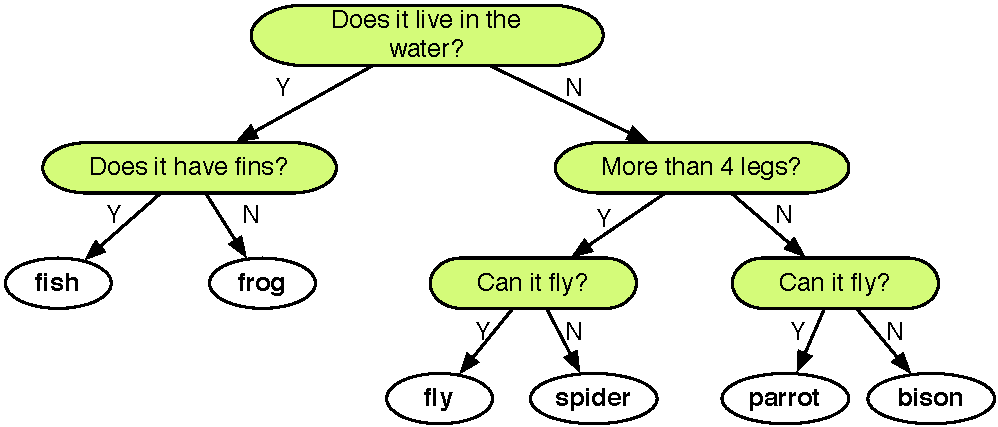
\includegraphics[scale=.6]{randomized/twentyquestion-game}
\end{center}

Interestingly, this strategy is optimal: There is no way you could have asked
any $2$ Yes/No questions to tell apart the $6$ possible answers.  If we can ask
only $2$ questions, any strategy that is deterministic and computes the output
using only the answers to these Yes/No questions can distinguish between only
$2^2 = 4$ possibilities.  Thus, using $3$ questions is the best one can do.


Determining the minimum number of questions necessary in the worst case in at
the crux of many lower-bound arguments. For starters, we describe a way to
represent a deterministic strategy for playing such a game in the definition
below.

\begin{definition}[Binary Decision Trees]
  A \emph{decision tree} is a tree in which
  \begin{itemize}
  \item each leaf node is an answer (i.e. what the algorithm outputs);
  \item each internal node represents a query---some question about the input
    instance---and has $k$ children, corresponding to one of the $k$ possible
    responses $\{0, \dots, k-1\}$;
  \item and the answer is computed as follows: we start from the root and follow
    a path down to a leaf where at each node, we choose which child to follow
    based on the query response.
  \end{itemize}
\end{definition}

The crucial observation is the following: If we're allowed to make at
most $q$
queries (i.e., ask at most $q$ Yes/No questions), the number of possible answers we can
distinguish is the number of leaves in a binary tree with depth at most $q$;
this is at most $2^q$.  Taking logs on both sides, we have
\begin{quote}
  \fbox{If there are $N$ possible outcomes, the number of questions needed is at least $\lg N$.}
\end{quote}
That is, there is \emph{some} outcome, that requires answering at least $\lg
N$ questions to determine that outcome.

\subsection{Warm-up: Guess a Number}

As a warm-up question, if I pick a number $a$ between $1$ and $2^{20}$, how
many Yes/No questions you need to ask before you can zero in on $a$?  By the
calculation above, since there are $N = 2^{20}$ possible outcomes, you will need
\emph{at least}
\[
\lg N = 20
\]
questions in the worst case.

Another way to look at the problem is to suppose I am devious and I
don't actually pick a number in advance.  Each time you ask a question
of the form ``is the number greater than $x$'', in effect you are
splitting the set of possible numbers into two groups.  I always answer
so the set of remaining possible numbers has the greater
cardinality. That is, each question you ask eliminates at most half of the
numbers.  Since there are $N = 2^{20}$ possible values, I can force you
ask $\lg N =20$ questions before I must  concede and pick the last remaining
number as my $a$.   This variation of the games shows that no matter what strategy
you use to ask questions, there is always \emph{some} $a$ that would cause you to
ask a lot of questions.

\subsection{A Sorting Lower Bound}

Let's turn back to the classical sorting problem.  We will prove
Theorem~\ref{thm:sorting-lb}. 

\begin{question}
Can you see how many comparisons would a sorting algorithm has to perform? 
\end{question}

A sorting algorithm must distinguish between all permutations of the
input, because in order to sort each, it has to perform something
different.  Connecting back to our decision tree diagram, the algorithm needs
 $\log(n!)$ queries to distinguish the $n!$ possible permutations (outcomes).


\begin{align*}
\log (n!) &= \log n + \log (n-1) + \dots + \log (n/2)+ \dots + \log 1 \\
&\geq \log n + \log (n-1) + \dots + \log (n/2) \\
&\geq \tfrac{n}{2} \cdot \log (n/2).
\end{align*}

 We can further improve the constants by applying Stirling's formula
  instead of this crude approximation.  Remember that \emph{Stirling's formula}
  gives the following approximation:
  \[ n! = \pparen{\frac{n}{e}}^n \sqrt{2\pi n}\pparen{1 + O(n^{-1})} > \pparen{\frac{n}e}^n,
  \]
  so $\lg (n!) > n \lg (n/e)$.



\subsection{A Merging Lower Bound}

Closely related to the sorting problem is the merging problem: Given two sorted
sequences $A$ and $B$, the merging problem is to combine these sequences into a
sorted one. To apply the argument we used for sorting, we'll need to count how
many possible outcomes the comparison operation can produce.

Suppose $n = |A|$, $m = |B|$, and $m \leq n$. We'll also assume that these
sequences are made up of unique elements. Now observe that we have not made any
comparison between elements of $A$ and $B$.  This means any interleaving
sequence $A$'s and $B$'s elements is possible.  Therefore, the number of
possible merged outcomes is the number of ways to choose $n$ positions out from
$n + m$ positions to put $A$'s elements; this is simply $\binom{n+m}{n}$.
Hence, we'll need, in the worst case, at least $\lg \binom{n+m}{n}$
comparison queries to merge these sequences.

The following lemma gives a simple lower bound for $\binom{n}{r}$, so that we
can simplify $\lg \binom{n+m}{n}$ to an expression that we recognize.

\begin{lemma}[Binomial Lower Bound]
  \[
\binom{n}{r} \geq \left(\frac{n}r\right)^r.
  \]
\end{lemma}
\begin{proof}
  First, we recall that
  \[
  \binom{n}{r} = \frac{n!}{r!(n-r)!} = \frac{n(n-1)(n-2)\dots(n-r+1)}{r(r-1)(r-2)\dots 1} =
  \prod_{i=0}^{r-1} \frac{n-i}{r-i}.
  \]
  We'll argue that for $0 \leq i < \min(r,n)$, $\frac{n-i}{r-i} \geq
  \frac{n}r$. Notice that
  \[
  \frac{n-i}{r-i} \geq \frac{n}r
  \iff r(n-i) \geq n(r-i)
  \iff rn - ri \geq nr - ni
  \iff (n-r)i \geq 0.
  \]
  Therefore, we have $\binom{n}r \geq \prod_{i=0}^{r-1} \frac{n-i}{r-i} \geq
  (n/r)^r$.
\end{proof}

With this lemma, we conclude that the number of comparison queries needed to
merge sequences of lengths $m$ and $n$ ($m \leq n$) is at least
\[
\lg \binom{n+m}{m} \geq m \lg \pparen{1 + \tfrac{n}m},
\]
proving Theorem~\ref{thm:merging-lb}

\end{comment}

\flushchapter
